\documentclass[11pt, a4paper]{article}
\usepackage[utf8]{inputenc} % encoding multi-byte
\usepackage[top=2.5cm, bottom=2.5cm, left=2.5cm, right=2.5cm]{geometry}
\usepackage{amsmath,amssymb,amsfonts,latexsym,textcomp} %paquetes matematicos
\usepackage{array,multirow,booktabs,tabulary} %tablas y arrays
\usepackage{graphicx}   
\usepackage{caption,float,subfigure} %float=figuras flotantes.
\usepackage{verbatim}  %texto raw 
\usepackage[ampersand]{easylist} %http://en.wikibooks.org/wiki/LaTeX/List_Structures#Easylist_package 
\usepackage{subfigure}
\usepackage{color}
\usepackage[usenames,dvipsnames,svgnames,table,x11names]{xcolor} 
%\usepackage{parskip}
%\setlength{\parindent}{0pt}	


%---- Bibliografia bibtex+biblatex -----------------------------------------
\usepackage[backend=bibtex,backref,natbib,sorting=none]{biblatex} %backref=hyperlinks de inversa, e.g.(vid. pag. xx)	
\bibliography{week5.bib} 

\usepackage{fancyhdr}
\pagestyle{fancy}
\fancyhf{}
\lhead{Registration Number: 180123717}
\cfoot{\thepage}
%---- tikz ----------------------------------------------------------------
\usepackage{tikz}
\usetikzlibrary{calc,patterns,angles,quotes,decorations.pathmorphing,decorations.markings,circuits,arrows,positioning,shapes}

%---- subsubequations numbering  -----------------------------------
%https://tex.stackexchange.com/questions/58489/nested-subequations-following-equations-get-wrong-numbers
\makeatletter
\newcounter{parentsubequation}% Counter for ``parent equation''.
\newenvironment{subsubequations}{%
	\refstepcounter{equation}%
	\protected@edef\theparentsubequation{\theequation}%
	\setcounter{parentsubequation}{\value{equation}}%
	\setcounter{equation}{0}%
	\def\theequation{\theparentsubequation\alph{equation}}%
	\ignorespaces
}{%
	\setcounter{equation}{\value{parentsubequation}}%
	\ignorespacesafterend
}
\makeatother


%---- Hyperlinks  ----------------------------------------------------------
\usepackage[ %
	breaklinks, %
	colorlinks=true, %
	linkcolor=black, %
	citecolor=black, %
	urlcolor=black %
]{hyperref} 
\urlstyle{same}

%---- Usar otros fonts + símbolo \degree -----------------------------------
\newcommand*{\myfont}{\fontfamily{lmtt}\selectfont}
\DeclareTextFontCommand{\textmyfont}{\myfont}	
\usepackage{gensymb} 

%---- Code highlighting con Listings ---------------------------------------
\usepackage{listings}	
\definecolor{mygreen}{rgb}{0.5,0.6,0.5}
\definecolor{mygray}{rgb}{0.5,0.5,0.5}
\definecolor{mymauve}{rgb}{0.58,0,0.82}
\definecolor{mygray2}{rgb}{0.9764, 0.9764, 0.9762}
%---- Config listings ------------------------------------------------------
\lstset{ %
	backgroundcolor=\color{mygray2},	% background color \color{mygray2}
	basicstyle=\footnotesize\ttfamily,	% tamaño de las letras y tipo de letra
	breaklines=true,	% corte de linea (line breaking)solo en espacio blanco
	captionpos=b,		% posicion del caption b,t,n (top,bottom,none)
	commentstyle=\color{ForestGreen},	% estilo del comentario
	%escapeinside={\%*}{*},	% si se desea agregar codigo Latex dentro el codigo debe ser %*codigo latex*
	frame=none,	% agrega marco al codigo (single)
	frameround=tttt,	% redondear el marco
	keepspaces=true,	% mantiene los espacios en el texto, util para mantener la indentacion del codigo (uso posible en columns=flexible)
	keywordstyle=\color{blue},	% estilo de los keywords
	stringstyle=\color{mymauve},	% estilo del string
	numbers=none,	% donde poner los numeros de linea, (none, left, right)
	numbersep=5pt,	% cuan lejos los numeros de linea estan del codigo
	xleftmargin=0pt,	% margen izquierdo
	showspaces=false,	% muestra espacios de codigo en todas partes usando el caracter barra baja "_", sobreescribe el comando 'showstringspaces'
	showstringspaces=false,	% muestra espacios solo en los strings
	tabsize=2,	% tabulacion por defecto =2
	title=\lstname	% muestra el nombre de lo archivos incluidos con \lstinputlisting; tambien se puede tratar con caption en vez de title
}	
%---- Config personalizada del caption -------------------------------------
\DeclareCaptionFont{white}{\color{black}}
\DeclareCaptionFormat{listing}{
%	\colorbox[cmyk]{0.43, 0.35, 0.35, 0.01 }{
%		\parbox{0.96\linewidth}{\hspace{15pt}#1#2#3}
%	}
	\colorbox{white}{
		\parbox{0.96\linewidth}{\centering #1#2#3}
	}
}
\captionsetup[lstlisting]{ format=listing, 
	labelfont=white, 
	textfont=white, 
	singlelinecheck=false, 
	margin=0pt, 
	font={bf,footnotesize} }
%---- Caracteres especiales ------------------------------------------------	
% Por defecto, listings no soporta inputec para mostrar los acentos y caracteres especiales.
% para manejar utf8 se debe enlistar los caracteres segun:
\lstset{literate=
	{á}{{\'a}}1 {é}{{\'e}}1 {í}{{\'i}}1 {ó}{{\'o}}1 {ú}{{\'u}}1
	{Á}{{\'A}}1 {É}{{\'E}}1 {Í}{{\'I}}1 {Ó}{{\'O}}1 {Ú}{{\'U}}1
	{à}{{\`a}}1 {è}{{\`e}}1 {ì}{{\`i}}1 {ò}{{\`o}}1 {ù}{{\`u}}1
	{À}{{\`A}}1 {È}{{\'E}}1 {Ì}{{\`I}}1 {Ò}{{\`O}}1 {Ù}{{\`U}}1
	{ä}{{\"a}}1 {ë}{{\"e}}1 {ï}{{\"i}}1 {ö}{{\"o}}1 {ü}{{\"u}}1
	{Ä}{{\"A}}1 {Ë}{{\"E}}1 {Ï}{{\"I}}1 {Ö}{{\"O}}1 {Ü}{{\"U}}1
	{â}{{\^a}}1 {ê}{{\^e}}1 {î}{{\^i}}1 {ô}{{\^o}}1 {û}{{\^u}}1
	{Â}{{\^A}}1 {Ê}{{\^E}}1 {Î}{{\^I}}1 {Ô}{{\^O}}1 {Û}{{\^U}}1
	{œ}{{\oe}}1 {Œ}{{\OE}}1 {æ}{{\ae}}1 {Æ}{{\AE}}1 {ß}{{\ss}}1
	{ç}{{\c c}}1 {Ç}{{\c C}}1 {ø}{{\o}}1 {å}{{\r a}}1 {Å}{{\r A}}1
	{ñ}{{\~n}}1 {£}{{\pounds}}1 {°}{{\degree}}1
}		
%---- Macro de inclusión de documentos con listings ------------------------
% [2]=numero de argumentos, #1=argumento 1, #2=argumento 2
\newcommand{\includecode}[2]{\lstinputlisting[language=#1, caption=#2, label=#2]{#2}}			
\renewcommand{\lstlistingname}{Code}
%=============================================================================================
%opening
\title{The University of Sheffield\\
	ACS6101 Foundations of Control Systems\\ 
	Week 5 Assignment}
\author{Paulo Roberto Loma Marconi\\ \url{prlomarconi1@sheffield.ac.uk}}
\date{November 4, 2018}

\begin{document}
\maketitle

\section{Question 1}
The aim of this task is to design a digital controlled system with some requirements, small steady state error, small settling time, minimum input action, and minimum overshoot. 

The plant to be studied is written as follows,
\begin{align}
G_p(s) &= \dfrac{0.04(s+1)}{s^2+0.2s+0.04} \\
\intertext{and the digital controller should have the form,}
D(z) &= K\dfrac{z-A}{z-B}
\end{align}

Fig.\ref{fig:Q1_Gp} shows that the plant is very slow and with a relatively big overshoot. Therefore, a phase margin ($PM$) of $60\degree$ can be the unique requirement. As long as the compensated phase margin is around that value, the settling time and overshoot should be minimized as much as possible.
 
\begin{figure}[H]
	\centering
	\subfigure[Bode plot]{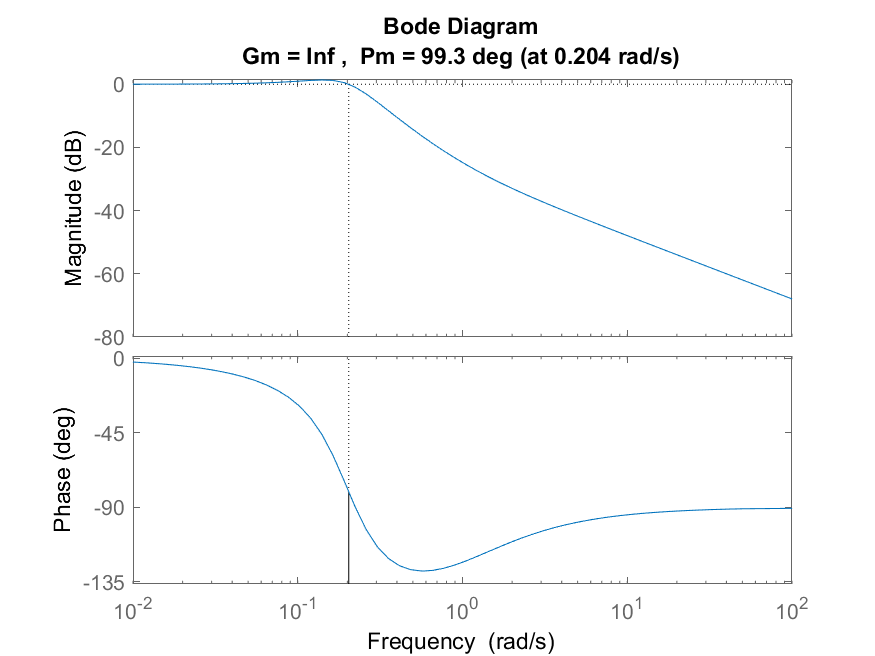
\includegraphics[width=0.48\linewidth]{../Q1_Gp_margin.png}}
	\subfigure[Step response.]{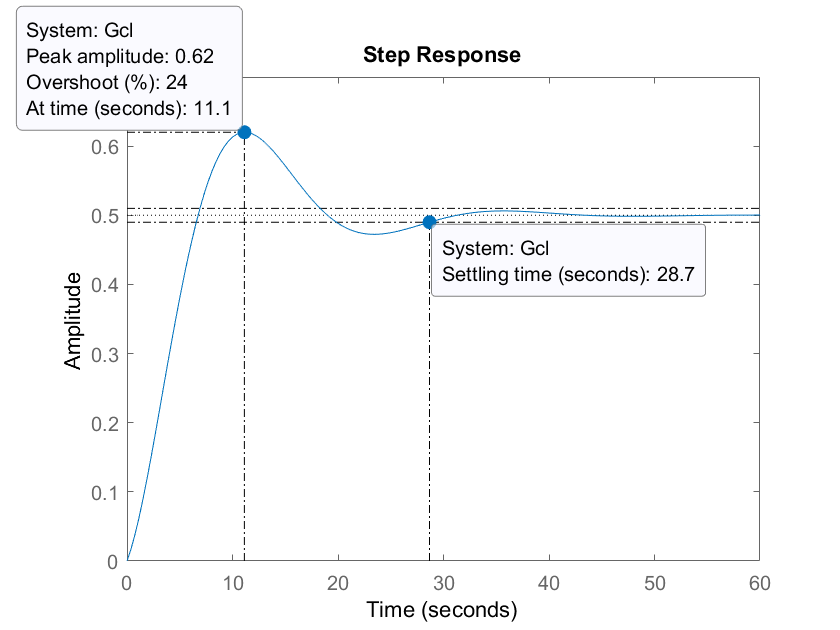
\includegraphics[width=0.48\linewidth]{../Q1_Gp_step_a.png}}
	\caption{Evaluation of the plant Gp}
	\label{fig:Q1_Gp}
\end{figure}


\subsection{Phase-Lead compensator}
The selected compensator can be written as follows,
\begin{align}
G_c = K_c~\dfrac{s+z}{s+p},\quad |z|\leq|p|
\end{align}

\textbf{Step 1.} Calculate a gain $K$ that satisfies the desired phase margin $PM_d=60\degree$. Applying the angle condition for a $PM_d$ over $G_p$,
\begin{align}
\measuredangle G_p(j\omega_c^\prime) &= PM_d - 180\degree \\
\measuredangle G_p(j\omega_c^\prime) &= 60\degree - 180\degree \nonumber\\
\measuredangle G_p(j\omega_c^\prime) &= -120\degree \nonumber
\end{align}
where $\omega_c^\prime$ is the new crossover frequency for the desired phase margin $PM_d=60\degree$.

Using the bode plot of $G_p$, Fig. \ref{fig:Q1_Gp_Gp1_bode}a, the logarithm gain at $-120\degree$ is $-8.02~dB$, so the gain $K$ can be calculated as follows,
\begin{align}
20\log_{10} K &= |-8.02|\\
K &= 2.52 \nonumber
\end{align}
Therefore, the uncompensated $G_p$ that satisfies the desired phase margin is,
\begin{align}
G_{p1} &= K~G_p \nonumber\\
G_{p1} &= 2.52 \dfrac{0.04(s+1)}{s^2+0.2s+0.04}
\end{align}
and Fig. \ref{fig:Q1_Gp_Gp1_bode}b shows that the new uncompensated plant $G_{p1}$ satisfies the desired phase margin.
 
\begin{figure}[H]
	\centering
	\subfigure[Bode plot of Gp]{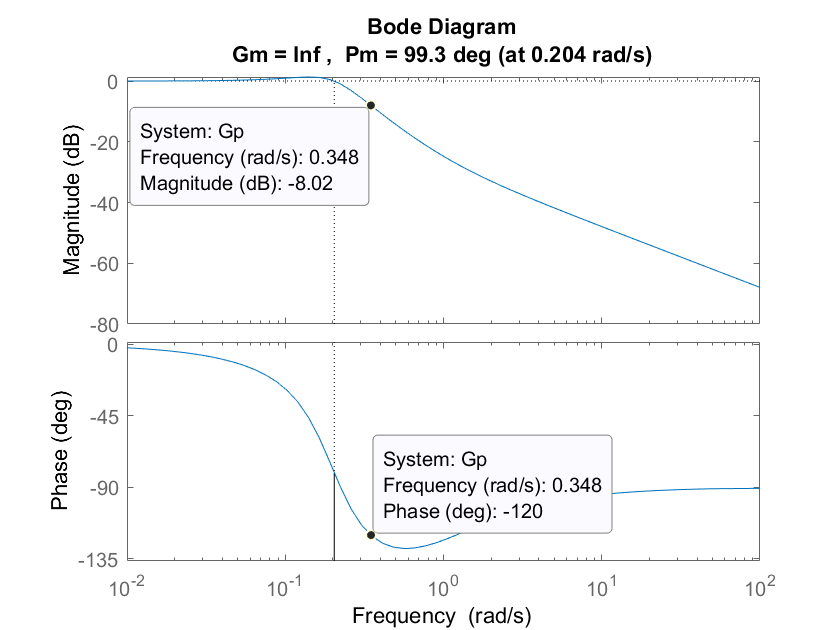
\includegraphics[width=0.48\linewidth]{../Q1_Gp_margin_a.png}}
	\subfigure[Bode plot of Gp1]{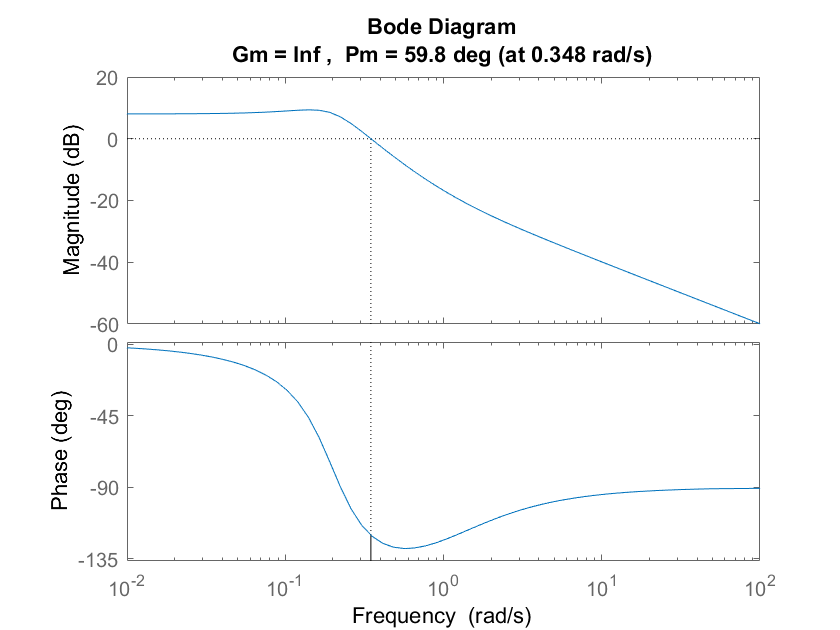
\includegraphics[width=0.48\linewidth]{../Q1_Gp1_K_margin.png}}
	\caption{Evaluation of the plant Gp and Gp1}
	\label{fig:Q1_Gp_Gp1_bode}
\end{figure}

The following Matlab scripts simulates the previous results.
\begin{lstlisting}[language=matlab, caption={}, label={}]
%% ========================================================================
% ---- ACS6101 Assignment week 5
% ---- Registration number: 180123717
% ---- Name: Paulo Roberto Loma Marconi
% ---- 03/11/2018
%% === Question 1 =========================================================
clear; clc; close all; % clean previous data in order to avoid erros.
%% plant Gp 
s = tf('s');
Gp = 0.04*(s+1)/(s^2+0.2*s+0.04); % uncompensated plant

fig = figure(1); 
margin(Gp); % calculates the phase margin and gain margin at their frequencies
[Gm,Pm,Wcg,Wcp] = margin(Gp);
Gcl = feedback(Gp,1); % closed-loop of the uncompensated plant
saveas(fig,'Q1_Gp_margin.png');

fig = figure(2);
step(Gcl); % step response to the closed-loop system
stepinfo(Gcl) % system performance values
saveas(fig,'Q1_Gp_step.png');
%% Design requirements
PO = 10; % percentage overshoot
zeta = log(100/PO)/sqrt(pi^2+ (log(100/PO))^2 ); % damping ratio
PM_d = round(100*zeta)+1; % desired PM
%% Obtaining the gain K that meets the desired PM_d
K = 10^(8.03/20); % the gain 8.03 obtained from the bode plot
Gp1 = K*Gp; % new uncompensated plant

fig = figure(11);
margin(Gp1);
saveas(fig,'Q1_Gp1_K_margin.png');
\end{lstlisting}

\textbf{Step 2.} The digital uncompensated $G_{z1}$ plant of $G_{p1}$ can be calculated using a zero-order holder with a sampling time $T_s=0.01$.
\begin{align}
G_{z1} &= 1.01\cdot10^{-3}\frac{z-0.99}{z^2-1.99z+0.99}
\end{align} 
In Fig. \ref{fig:Q1_Gz1_K_step} it can be seen that the continuous and discrete plant are almost similar. Also, the settling time has been reduced but the steady state error is too big.

\begin{figure}[H]
	\centering
	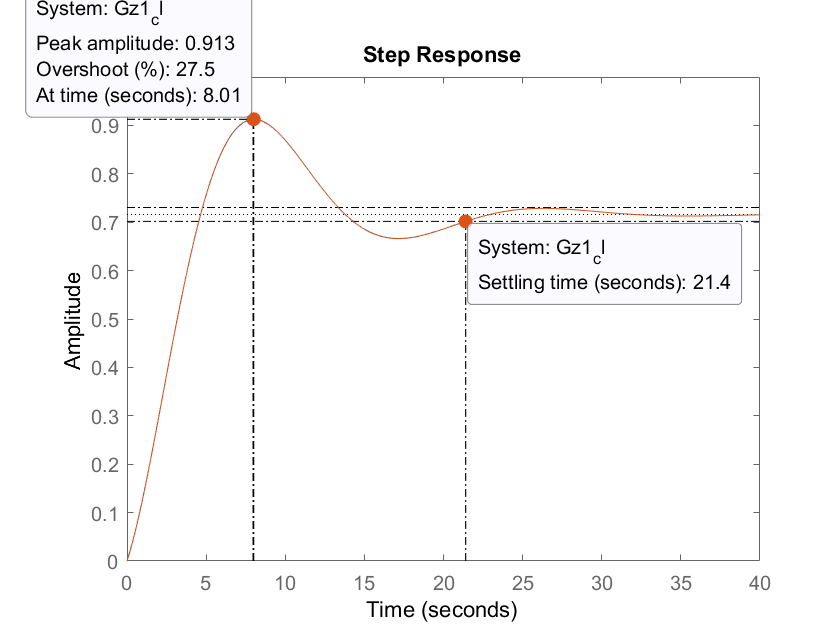
\includegraphics[width=0.48\linewidth]{../Q1_Gpz_K_step_a.png}
	\caption{Step response of Gz1 and Gp1}
	\label{fig:Q1_Gz1_K_step}
\end{figure}

\textbf{Step 3.} With the desired phase margin, the value of $\beta$ can be calculated as follows,
\begin{align}
PM_{act}- & PM_d+\theta = \arctan\dfrac{\beta-1}{2\sqrt{\beta}}
\end{align}
where $PM_{act}$ is the actual phase margin of the uncompensated plant $G_{p1}$, and $\theta$ is a factor of correction.

After some operations,
\begin{align}
\beta^2- & \beta\left[2+4\left(\tan(PM_d-PM_{act}+\theta)\right)\right] +1 = 0 \nonumber\\
\intertext{if $\theta=6\degree$, $PM_d=60\degree$, and $PM_{act}=61.25\degree$ obtained from Fig. \ref{fig:Q2_Gp2_margin}, $\beta$ will be,}
&\qquad \beta = 1.18 \nonumber
\end{align}

\begin{figure}[H]
	\centering
	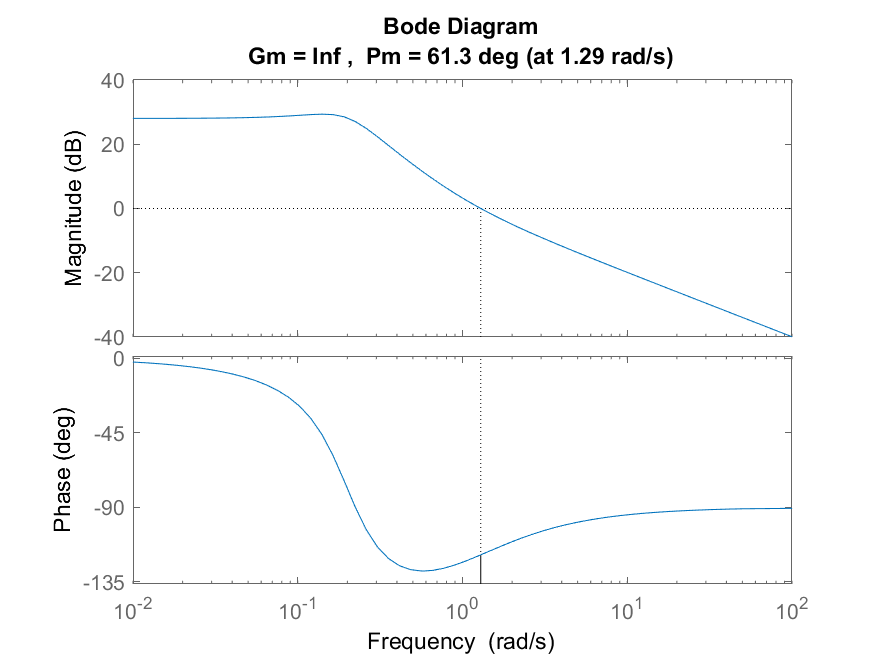
\includegraphics[width=0.48\linewidth]{../Q1_Gp2_margin.png}
	\caption{Bode plot of Gp2}
	\label{fig:Q2_Gp2_margin}
\end{figure}


\textbf{Step 4.} Now, the  crossover over frequency $\omega_c$ needs to be calculated using the following gain condition formula,
\begin{align}
\left| G_{p1}(j\omega_c) \right| &= \dfrac{1}{\sqrt{\beta}} \\
\intertext{if we use the peak magnitude $M_{pc}$ relation,}
M_{pc} &= \dfrac{1}{\sqrt{\beta}} \\
\intertext{and using \texttt{getGainCrossover(Gp2,Mpc)} on Matlab,}
\omega_c& = 1.37 ~rad/sec \nonumber
\end{align}

\textbf{Step 5.} Determining the zero of the controller,
\begin{align}
\omega_c &= \sqrt{\beta z^2}\\
z &= 1.26 \nonumber\\
\intertext{therefore, the compensator in continuous time can be written as follows,}
G_c &= \beta\dfrac{s+z}{s+\beta z} \\
G_c &= 1.18~\dfrac{s+1.26}{s+1.49} \nonumber\\
\intertext{and in discrete time,}
G_cz &= 1.18~\dfrac{z-0.99}{z-0.98} \nonumber\\
\intertext{The open-loop compensated in continuous and discrete time are,}
G_{ol} &= G_c~ G_{p1}\\
G_{ol} &= 1.18\quad\dfrac{s+1.26}{s+1.49} \quad 2.52\quad\dfrac{0.04(s+1)}{s^2+0.2s+0.04} \\
G_{olz} &= 0.01\quad \dfrac{z-0.99}{z-0.98}\quad\dfrac{z-0.98}{z^2-1.99+0.99}
\end{align}
 
Fig. \ref{fig:Q1_lead} shows that the compensated system using a Phase-Lead controller achieves with success the desired phase margin of $60\degree$, and has a small settling time $t_s=4.84~sec$.

\begin{figure}[H]
	\centering
	\subfigure[Bode plot]{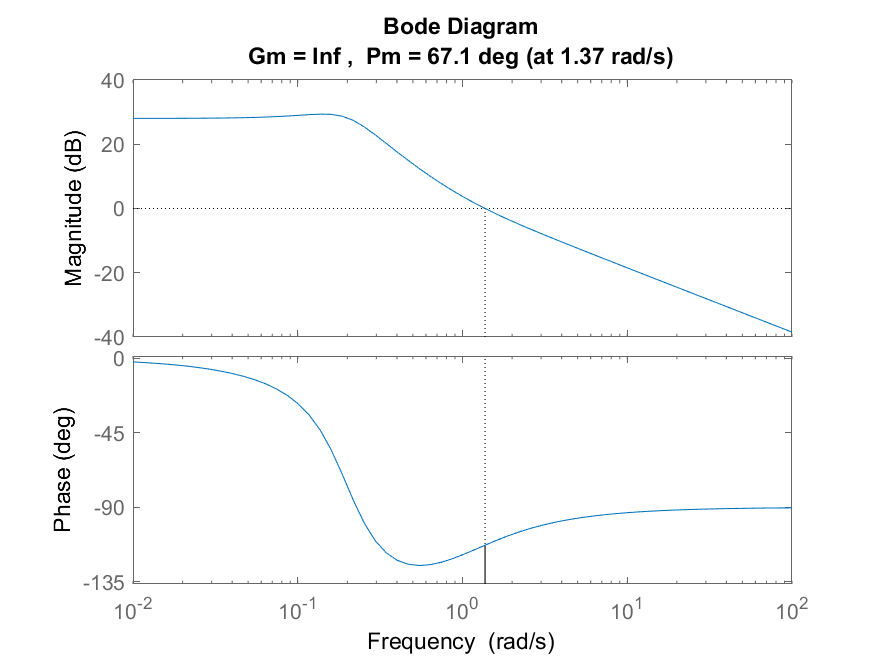
\includegraphics[width=0.48\linewidth]{../Q1_lead_margin.png}}
	\subfigure[Step response.]{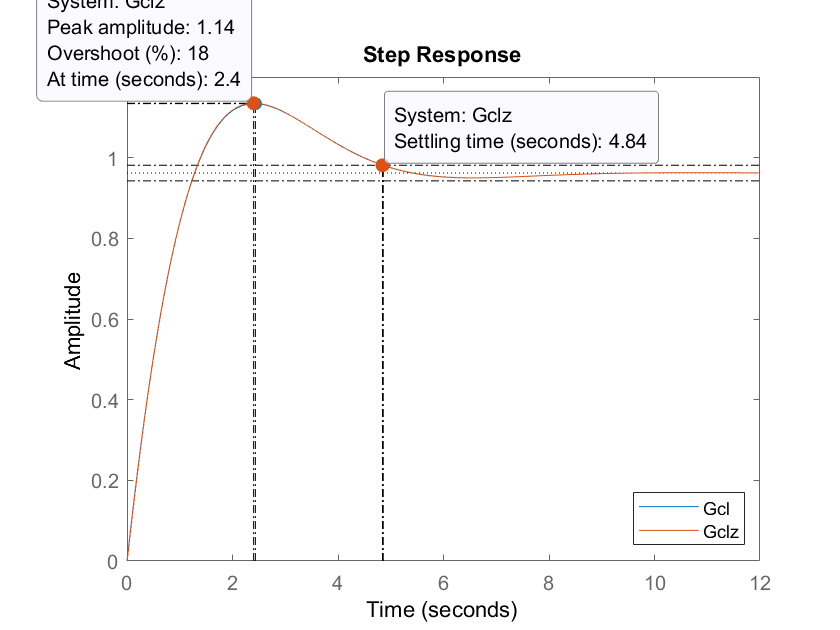
\includegraphics[width=0.48\linewidth]{../Q1_lead_step_a.png}}	
	\caption{Evaluation of Phase-Lead compensated system in continuous and discrete time.}
	\label{fig:Q1_lead}
\end{figure}

The following Matlab script simulates and evaluates the previous design.
\begin{lstlisting}[language=matlab, caption={}, label={}]
%% Designing the Phase-lead digital controller 
% introducing a new gain 10 times faster in ordert to obtain a fast
% response to the step input
Gp2 = K*10*Gp;

fig = figure(4);
margin(Gp2); % checking the desired phase margin PM_d 
[Gm1,PM_act,Wcg1,Wcp1] = margin(Gp2);
saveas(fig,'Q1_Gp2_margin.png');

% step 1) obtaining beta with the actual PM and the desired PM
theta = 6; % correction factor
beta = roots( [1 -(2+4*( tand(PM_d-PM_act+theta) )^2) 1] );
% beta = (1+sind(PM_d-PM_act+theta))/(1-sind(PM_d-PM_act+theta));
% step 2) calculating the new crossover frequency
Mpc = 1/sqrt(beta(1)); % find compensator peak magnitude.
omega_c = getGainCrossover(Gp2,Mpc); % The new gain crossover frequency wc
% step 3) determining the zero and the pole of the controller
zc = omega_c/sqrt(beta(1)); % zero of the controller
pc = beta(1)*zc; % pole of the controller
% step 4) controller in continuous and discrete time
Gc = beta(1)*(s+zc)/(s+pc); % phase-lead controller in continuous time
Gcz = c2d(Gc,Ts,'zoh'); % phase-lead controller in discrete time
%% Evaluating the phase-lead controller
Gol = Gc*Gp2; % open-loop compensated in continuous time
Gcl = feedback(Gol,1); % closed-loop in continuous time
Gp2z = c2d(Gp2,Ts,'zoh'); % plant in discrete time
Golz = Gcz*Gp2z; % open-loop compensated in discrete time
Gclz = feedback(Golz,1); % closed-loop in discrete time

fig = figure(5);
margin(Gol);
saveas(fig,'Q1_lead_margin.png');

fig = figure(6);
step(Gcl,Gclz);
saveas(fig,'Q1_lead_step.png');
\end{lstlisting}

\section{Question 2}
The deadbeat controller is a type of controller that reaches zero error very fast at the sampling instants in the discrete domain systems, but it can not be used in continuous time, \cite{Westphal2012}. Another characteristics are that the control signal is very high, and the overshoot is less than 2\%.

As long as the plant $G(z)$ has all zeros and poles inside the unit circle (minimum phase), the plant can be written as,
\begin{align}
G(z) &= \dfrac{z^{d} B(z)}{A(z)} = \dfrac{z^{d}(b_o + b_1 z^{-1}+...+b_m z^{-m})}{1+a_1 z^{-1} + ... + a_n z^{-n}}, \quad d=n-m>0
\end{align}
the digital deadbeat will have the following transfer function,
\begin{align}
D(z) &= \dfrac{A(z)}{z^{-d}B(z)}~\dfrac{z^{-d}}{1-z^{-d}}\\
\intertext{and the closed-loop system is,}
Y(z) &= z^{-d} U(z)
\end{align}


The aim of this question is to design a digital deadbeat controller for the plant,
\begin{align}
G_p(s) &= \dfrac{0.04(s+1)}{s^2+0.2s+0.04} \\
G_p(z) &= \dfrac{5.47\cdot 10^{-2}(z-0.34)}{z^2 - 1.78z + 0.82}
\end{align}
with a the sampling time $T_s=1$.

After using the following code in Matlab.
\begin{lstlisting}[language=tex, caption={}, label={}]
%% ========================================================================
% ---- ACS6101 Assignment week 5
% ---- Registration number: 180123717
% ---- Name: Paulo Roberto Loma Marconi
% ---- 03/11/2018
%% === Question 2 =========================================================
clear; clc; close all;
s = tf('s');
Gp = 0.04*(s+1)/(s^2+0.2*s+0.04); % uncompensated plant
Ts = 1; % sampling time
Gz = c2d(Gp,Ts,'zoh'); % System transfer function in discrete time
% Minimum phase case
z=zpk('z',Ts);
Mz = 1/z; % closed-loop because the relative order d = 1
Dz = Mz/(Gz*(1-Mz)); % deadbeat controller
Dz = minreal(Dz); % cancel common factors
fig = figure(1); 
step(Dz*Gz/(1+Dz*Gz)) % step response of closed-loop
saveas(fig,'Q2_deadbeat_step.png');
fig = figure(2); 
step(Dz/(1+Dz*Gz)) % control signal
saveas(fig,'Q2_deadbeat_control.png');
\end{lstlisting}

The closed-loop discrete system is as follows,
\begin{align}
G_{clz} &= \dfrac{(z-1) (z-0.3392)^2 (z^2 - 1.783z + 0.8187)^2} {z (z-0.3392)^2 (z-1) (z^2 - 1.783z + 0.8187)^2} \\
\intertext{where the controller is,}
G_{cz} &= \dfrac{18.288 (z-1) (z-0.3392) (z^2 - 1.783z + 0.8187)^2}{z (z-0.3392)^2 (z-1) (z^2 - 1.783z + 0.8187)}
\end{align}

Fig. \ref{fig:Q2_deadbeat} shows the output of the deadbeat controller and the closed-loop system response to a unit step input. It shows clearly that the steady-state error reaches zero value at the first sampled time.

In addition, the control signal is very high when the sampling time is increased, Fig. \ref{fig:Q2_deadbeat_a}.

\begin{figure}[H]
	\centering
	\subfigure[Step response of the closed-loop]{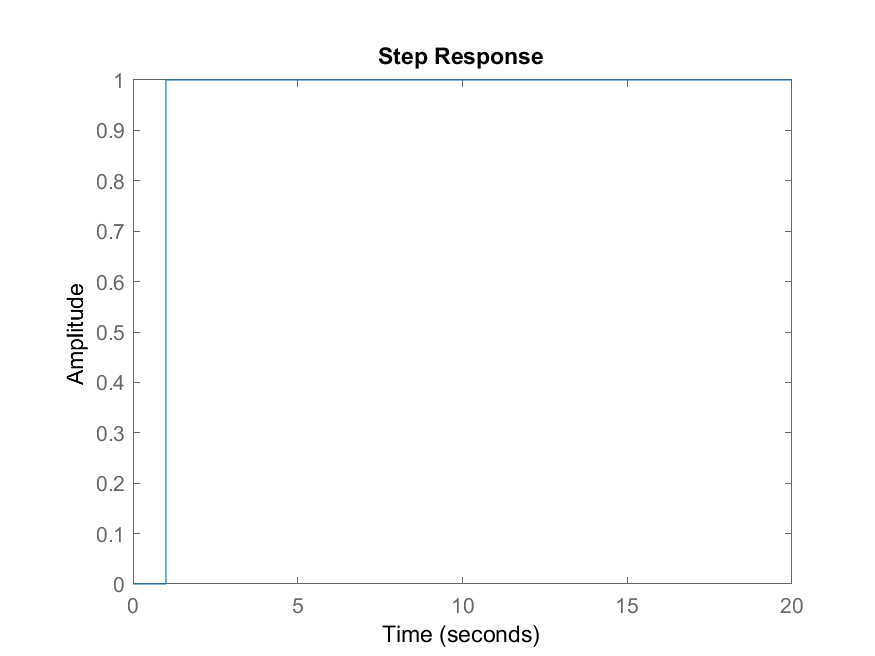
\includegraphics[width=0.48\linewidth]{../Q2_deadbeat_step.png}}
	\subfigure[Control signal]{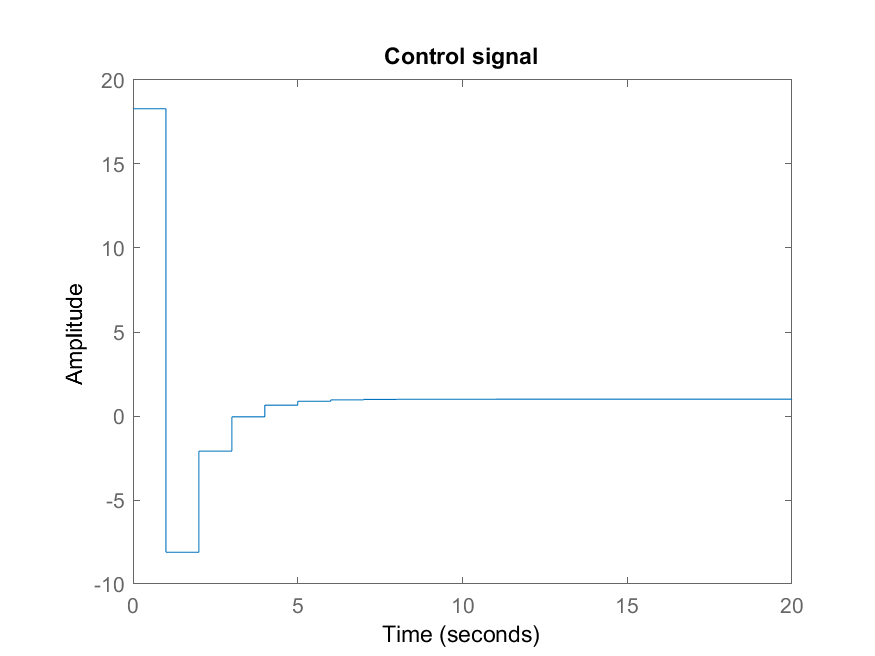
\includegraphics[width=0.48\linewidth]{../Q2_deadbeat_control.png}}
	\caption{Performance of the deadbeat controller system for $T_s=1$}
	\label{fig:Q2_deadbeat}
\end{figure}



\begin{figure}[H]
	\centering
	\subfigure[Step response of the closed-loop]{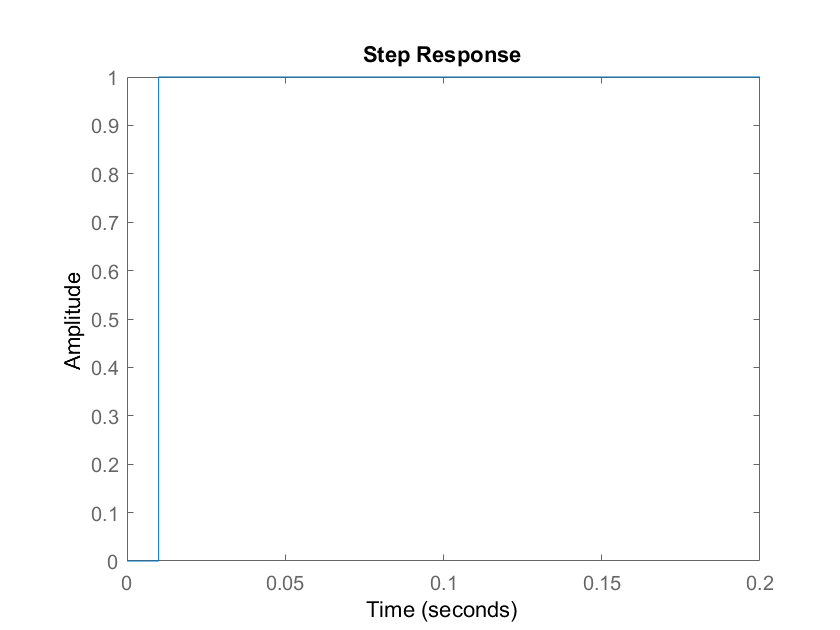
\includegraphics[width=0.48\linewidth]{../Q2_deadbeat_step_a.png}}
	\subfigure[Control signal]{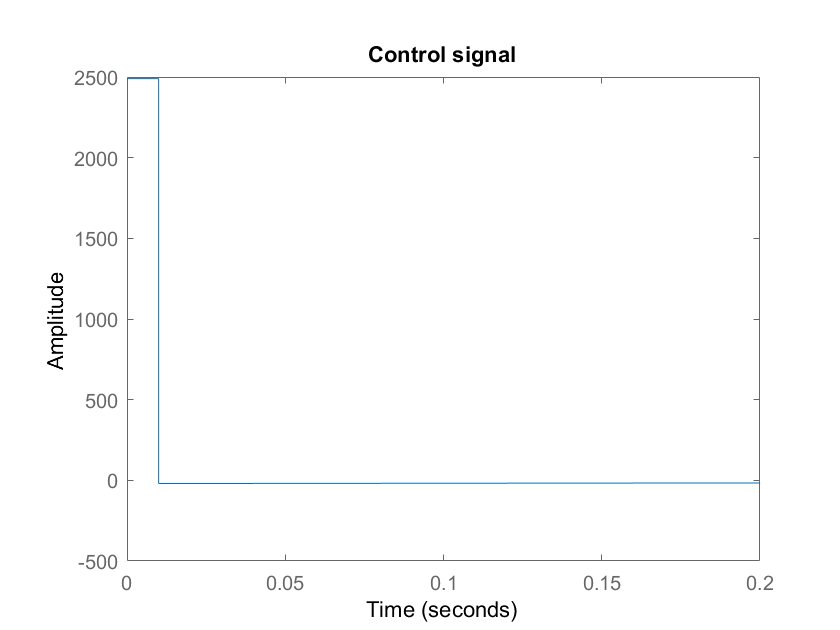
\includegraphics[width=0.48\linewidth]{../Q2_deadbeat_control_a.png}}
	\caption{Performance of the deadbeat controller system for $T_s=0.01$}
	\label{fig:Q2_deadbeat_a}
\end{figure}


\printbibliography
\end{document}
